% !TeX spellcheck = cs_CZ
{\tikzset{external/prefix={tikz/CES/}}
 \tikzset{external/figure name/.add={ch07_}{}}
%---------------------------------------------------------------------------------------------------
% file AVR_MCU.tex
%---------------------------------------------------------------------------------------------------
%============================== Kapitola: Procesory AVR=============================================
\chapter{Procesory AVR}
\minitoc

\section{AVR Architektura}
  Mikroprocesory AVR, obdobně jako např. řada '51, mají \emph{Harvardskou architekturu} (viz 
  kapitola \ref{ces:IchapIVsecIssecIII}), tzn. že paměť programu a paměť dat jsou odděleny. 
  Základní rozdělení paměťového prostoru je na \ref{ces:fig001}.

  \begin{figure}[ht!]  %\ref{ces:fig001}
    \centering
    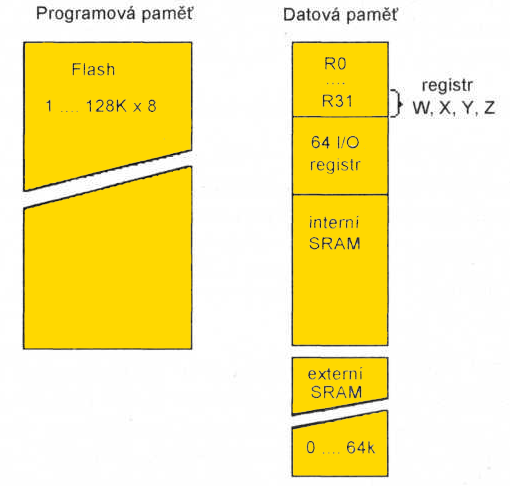
\includegraphics[width=0.6\linewidth]{ces_fig001.png}
    \caption{Paměťová mapa AVR mikroprocesorů
            (\cite[s.~7]{Subert2002})}
    \label{ces:fig001}
  \end{figure}
  
  Pro zpracování instrukce se používá \emph{pipeline} (zřetězené zpracování), kdy v době vykonání 
  instrukce se následující instrukce vyčítá z paměti a připravuje ke zpracování.  Proto je většina 
  instrukcí provedena v jednom hodinovém cyklu.
  
  AVR architektura vychází z koncepce rychle přístupného registrového pole, které obsahuje 32 
  obecně použitelných registrů délky 8 bitů. Přístup do registrového pole je proveden v jediném 
  strojovém cyklu. To znamená, že během jednoho strojového cyklu lze vykonat jednu 
  aritmeticko-logickou operaci\footnote{oba operandy aritmeticko-logické operace jsou načteny z 
  registrového pole, operace je provedena a výsledek směřuje opět do registrového pole v jediném 
  strojovém cyklu}

  Tato technika, umožňuje vyšší výkon ve srovnání s mikrokontroléry řady 8051, které disponují 
  instrukcemi o délce od 12 do 48 hodinových cyklů, navíc se pro výpočty musí používat 
  akumulátor, který je jen jeden. Registrové pole lze v tomto smyslu chápat jako skupinu 
  akumulátorů.

  \subsection{Strojový cyklus}
    Strojový cyklus mikrokontrolérů AVR přímo odpovídá hodinovému cyklu. Nedochází k žádnému 
    dělení  hodinových cyklů jako například u mikrokontrolérů řady 8051\footnote{jeden strojový 
    cyklus obsahuje 12 hodinových cyklů}
  \subsection{Prefetch a pipelining}
    Mikrokontroléry AVR používají jednoduchý \emph{předvýběr instrukce} (\textbf{prefetch}) 
    umožňující \emph{jednofázové zřetězení instrukcí} (\textbf{pipe\-lining})

} % tikzset
%---------------------------------------------------------------------------------------------------
\printbibliography[title={Seznam literatury}, heading=subbibliography]
\addcontentsline{toc}{section}{Seznam literatury}